\documentclass[thesis]{subfiles}

\begin{document}

\chapter{Context of this work}

\section{Flexible nanoporous materials}

\subsection{Porous materials}

Porous materials are material presenting a structural porosity, their
tri-dimensional structure showing cavities called \emph{pores}. This pores
network can vary in homogeneity and regularity, creating a wide variety of
porous materials. They all have in common a high specific surface area, which is
the accessible internal surface by grams of the material --- up to thousands of
square meters by gram of material\cite{Farha2012} in the most extreme cases.
This very high specific surface area of porous materials is exploited in a
number of important industrial applications, especially in the domains of
adsorption and catalysis. For example, porous materials are used to separate
gases in mixtures as molecular sieves; to filter and remove heavy metals from
water; or in heterogeneous catalysis in oil refineries by the cracking process.

The International Union for Pure and Applied Chemistry (IUPAC) recommends to
classify porous materials in three groups, depending on the size of the
pores\cite{Rouquerol1994}. First are the \emph{microporous} solids, where the
pores are less than \SI{2}{nm} in diameter. Then we find the \emph{mesoporous}
solids with pore diameter between 2 and \SI{50}{nm}. Porous solids with pores
larger than \SI{50}{nm} are called \emph{macroporous} solids. Microporous and
mesoporous solids are often grouped together as \emph{nanoporous} solids, where
the size of pores does not exceed \SI{50}{nm}.

\begin{figure}[ht]
    \centering
    \raisebox{-0.5\height}{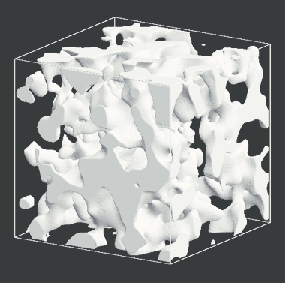
\includegraphics[width=0.3\textwidth]{figures/images/porous-vycor}}
    \hfill
    \raisebox{-0.5\height}{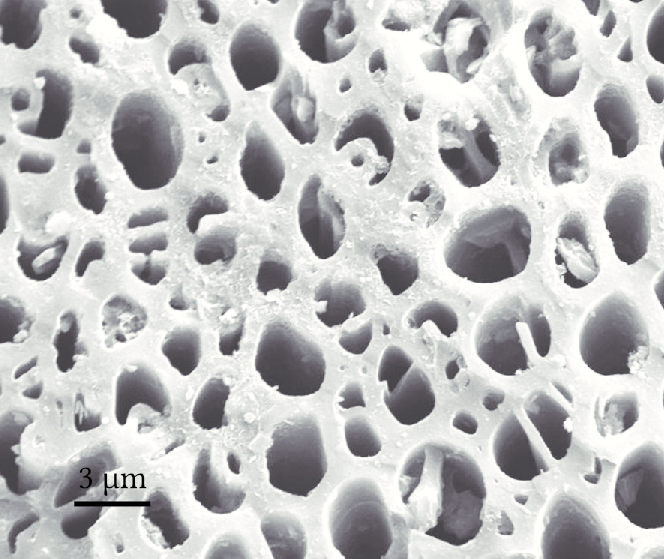
\includegraphics[width=0.3\textwidth]{figures/images/porous-carbon}}
    \hfill
    \raisebox{-0.5\height}{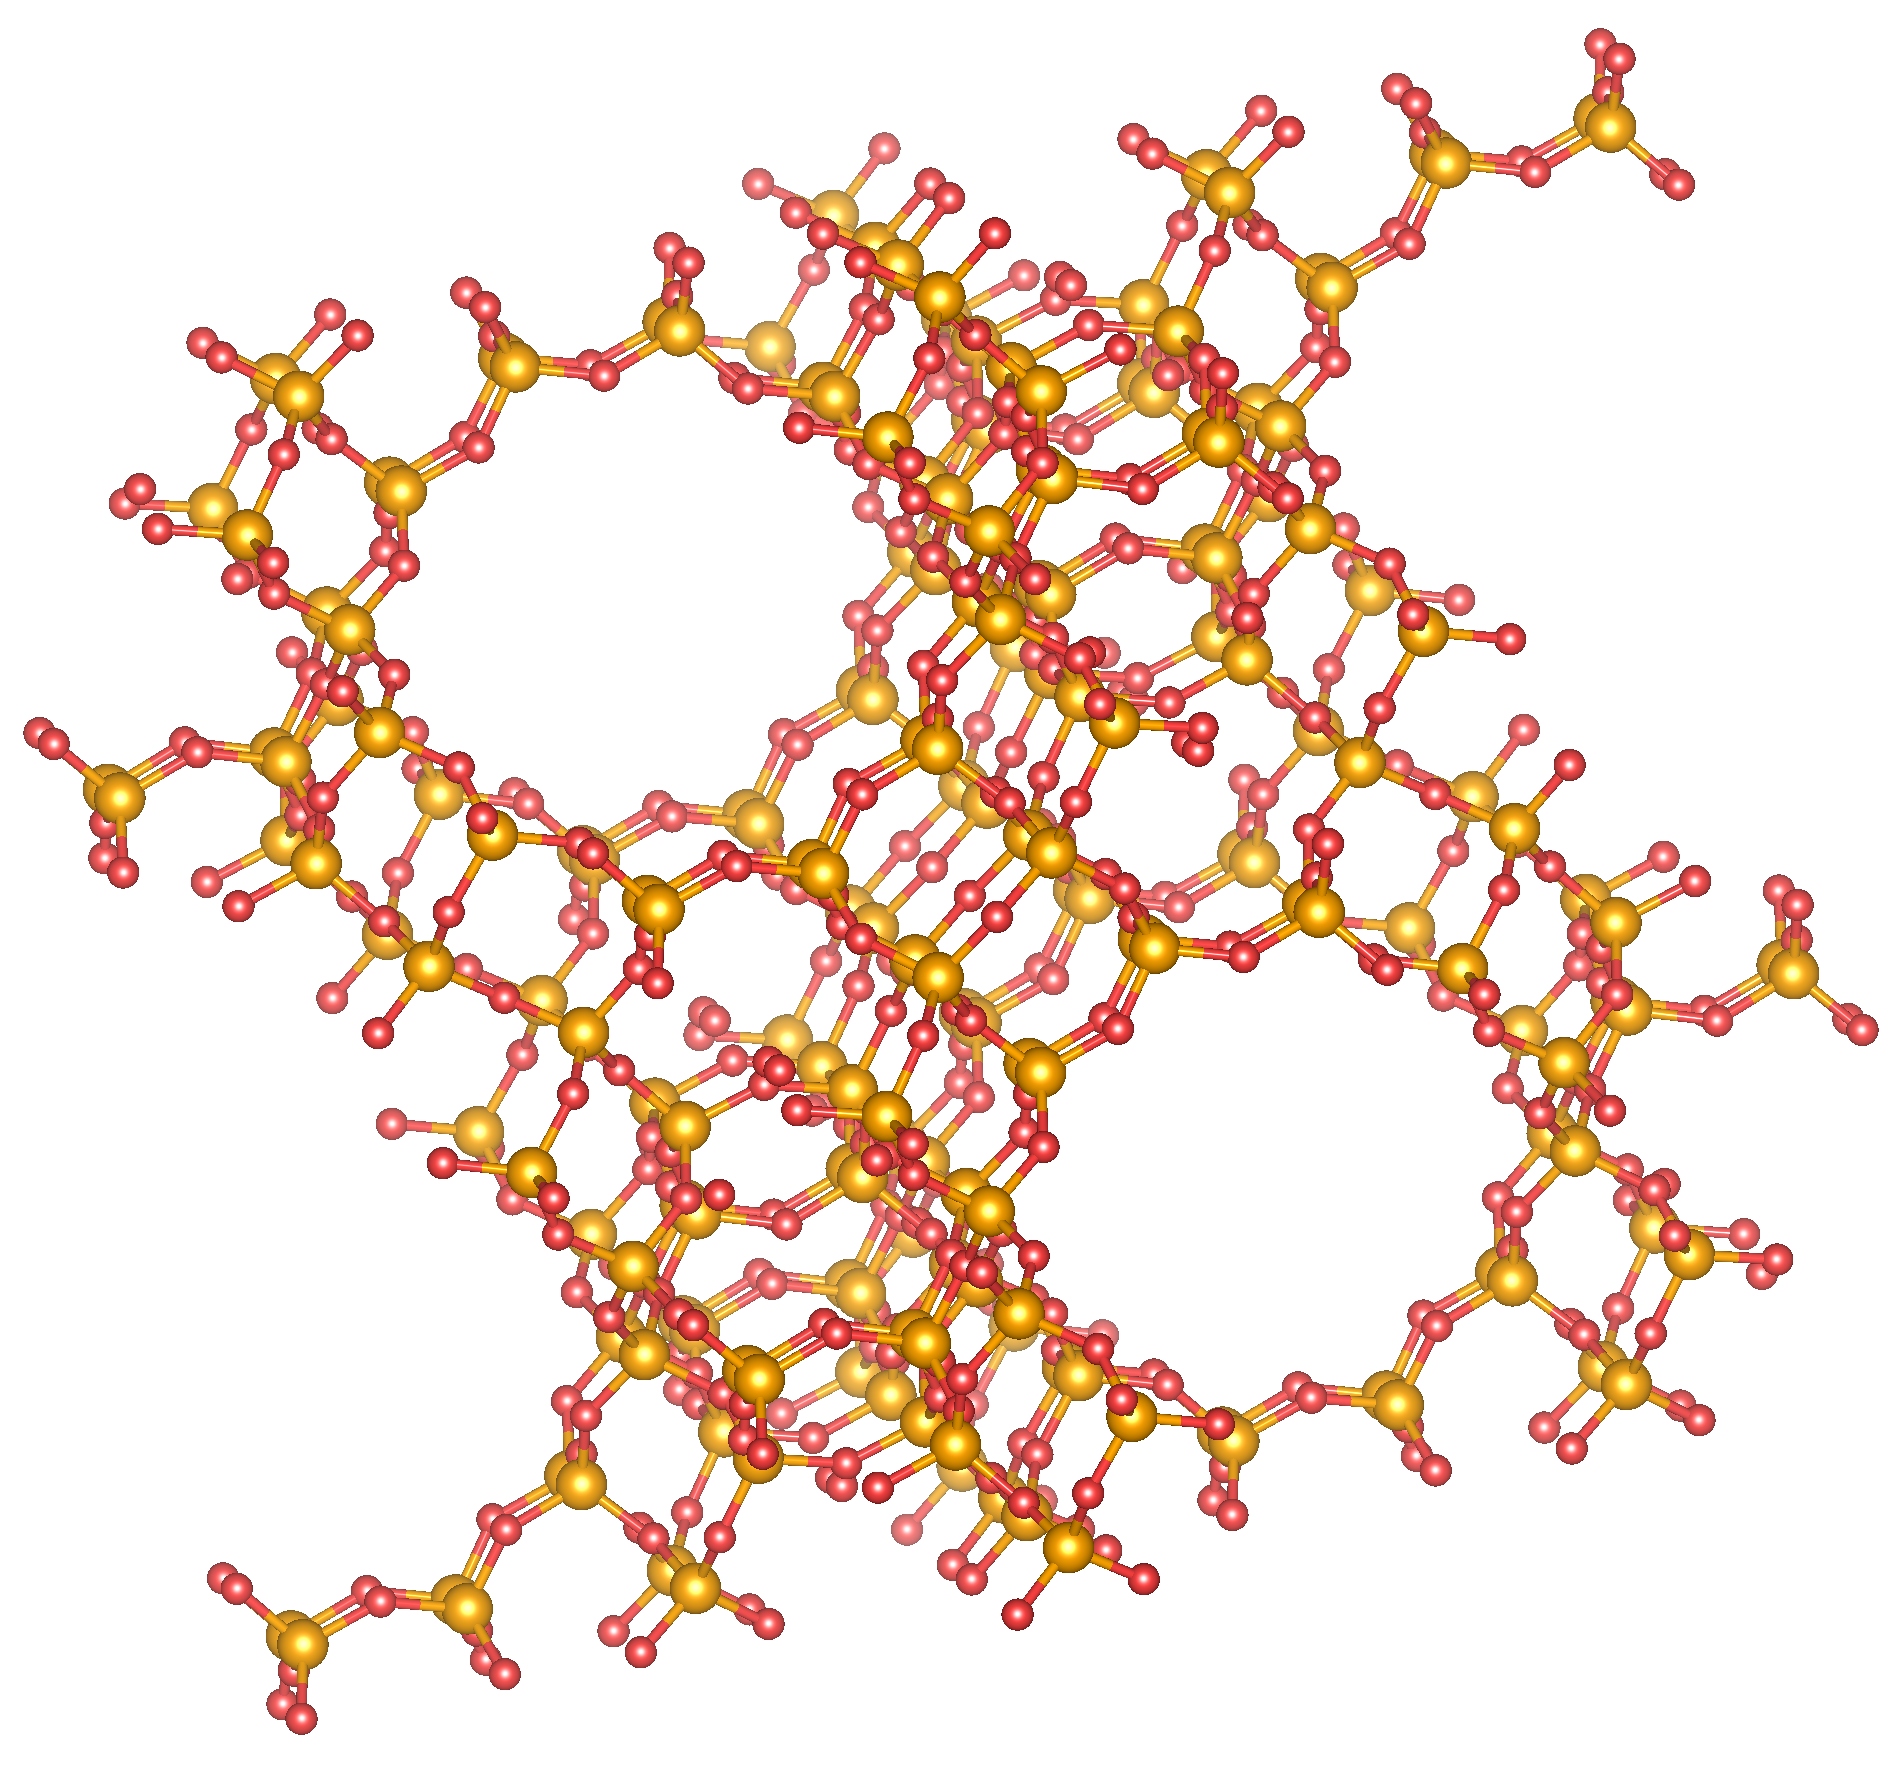
\includegraphics[width=0.3\textwidth]{figures/images/porous-faujasite}}
    \caption{Three examples of porous material. The left image is a
    representation of a vycor glass (disordered)\cite{Levitz2003}; the middle
    is a scanning electron microscope image of activated carbon (ordered but non
    crystalline)\cite{TODO}; and right is the crystalline structure of the
    zeolite faujasite.}
    \label{fig:porous-examples}
\end{figure}

Porous materials are also classified depending on their structural regularity,
from highly regular crystalline materials such as zeolites and
\emph{Metal-Organic Frameworks} (MOFs) showing a periodic organization of their
atoms; to regular porous materials such as clays and carbon nanotubes, where the
porosity is well defined but does not present long-distance ordering. Finally,
there also exist amorphous porous materials, which have a wide distribution of
pore sizes and shapes, an no periodicity. Examples in this latter class are
vycor glasses, silica glasses, or aerogels. Three example of porous solids with
different pore size and regularity are presented in
figure~\ref{fig:porous-examples}.

A final distinction we can make among porous materials is the one of their
chemical nature. They are usually classified as either organic or inorganic
materials. The former contains materials build around carbon atoms, such as
carbon nanotubes, or porous polymers. The latter class have historically been
the widest one, containing materials such as oxides, alumino-silicates, sulfurs
compound or alumino-phosphates. In the last few decades, we have seen blooming a
new class of materials, with an hybrid inorganic-organic composition. This new
family contains organo-silicic material, and \emph{Metal-Organic Frameworks}
which have been the main subject of study in my PhD.

During my PhD, I studied hybrid inorganic-organic crystalline nanoporous
materials, and especially flexible ones. In the next sections, I will describe
zeolites as the conventional example of crystalline porous material, and MOFs as
the relatively new class of hybrid inorganic-organic porous materials. I will
also present the \emph{Zeolitic Imidazolate Framework} (ZIF) family of MOFs,
which are MOFs with a zeolite topology.

\subsection{Zeolites}
\subsubsection{Structure and composition}

\begin{figure}[ht]
    \centering
    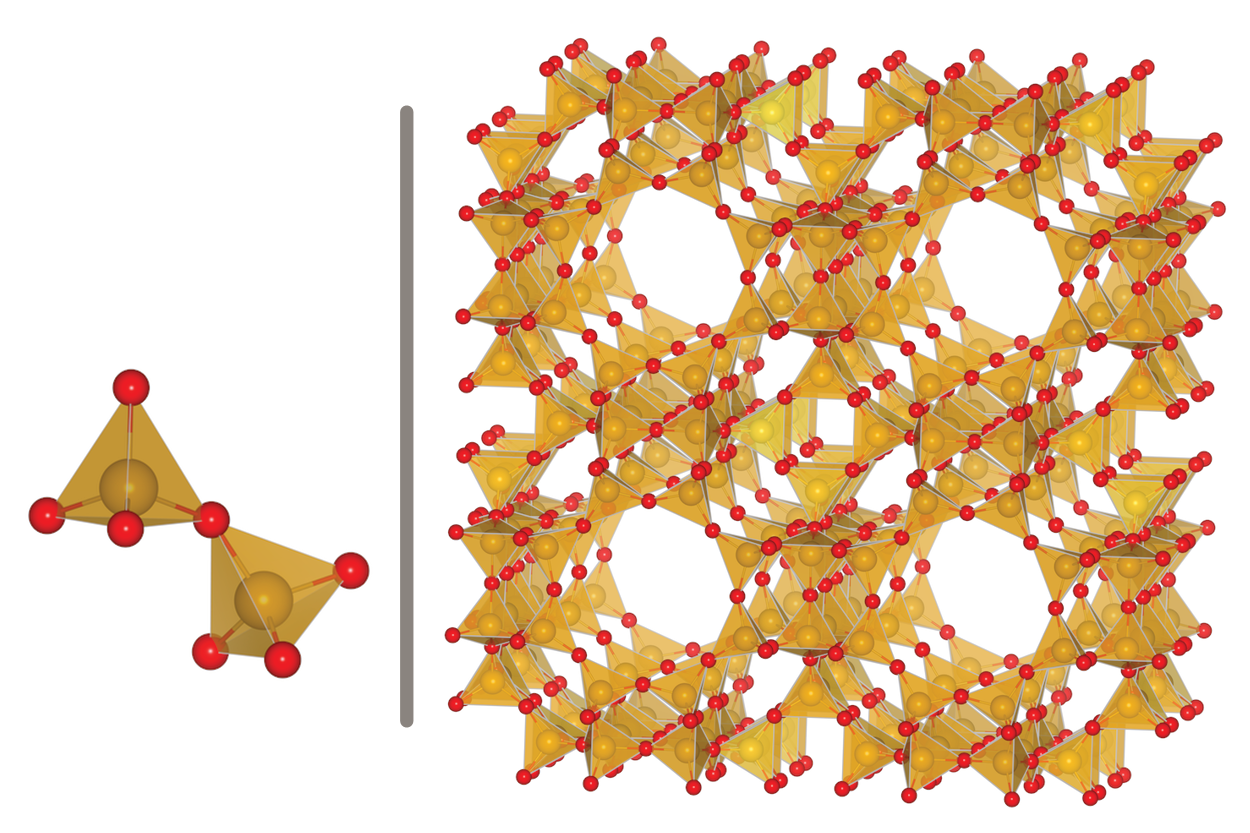
\includegraphics[width=0.8\textwidth]{figures/images/zeolite-building-blocks}
    \caption{Two \ce{SiO4} tetrahedra on the right, and the structure of zeolite
    LTA on the left. Si atoms are in yellow and oxygen atoms in red.}
    \label{fig:zeolite-building-block}
\end{figure}

\subsection{Metal organic frameworks}

\begin{figure}[ht]
    \centering
    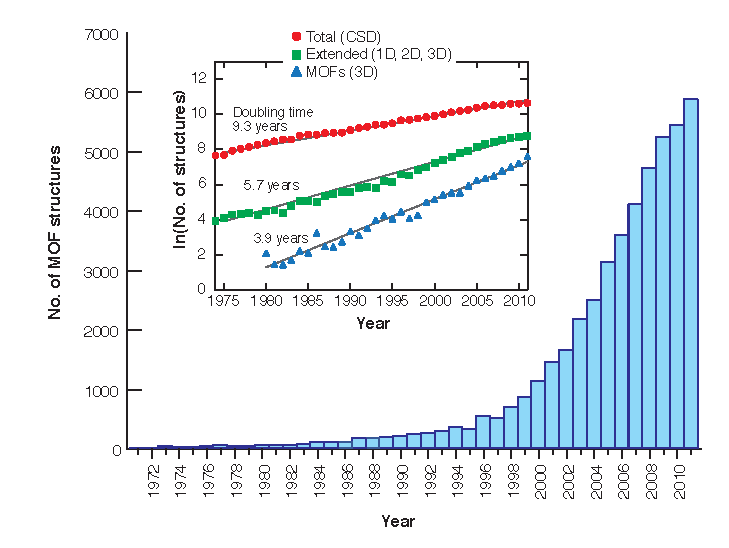
\includegraphics[width=0.7\textwidth]{figures/images/number-of-mofs}
    \caption{\TODO}
    \label{fig:number-of-mofs}
\end{figure}

\begin{figure}[ht]
    \centering
    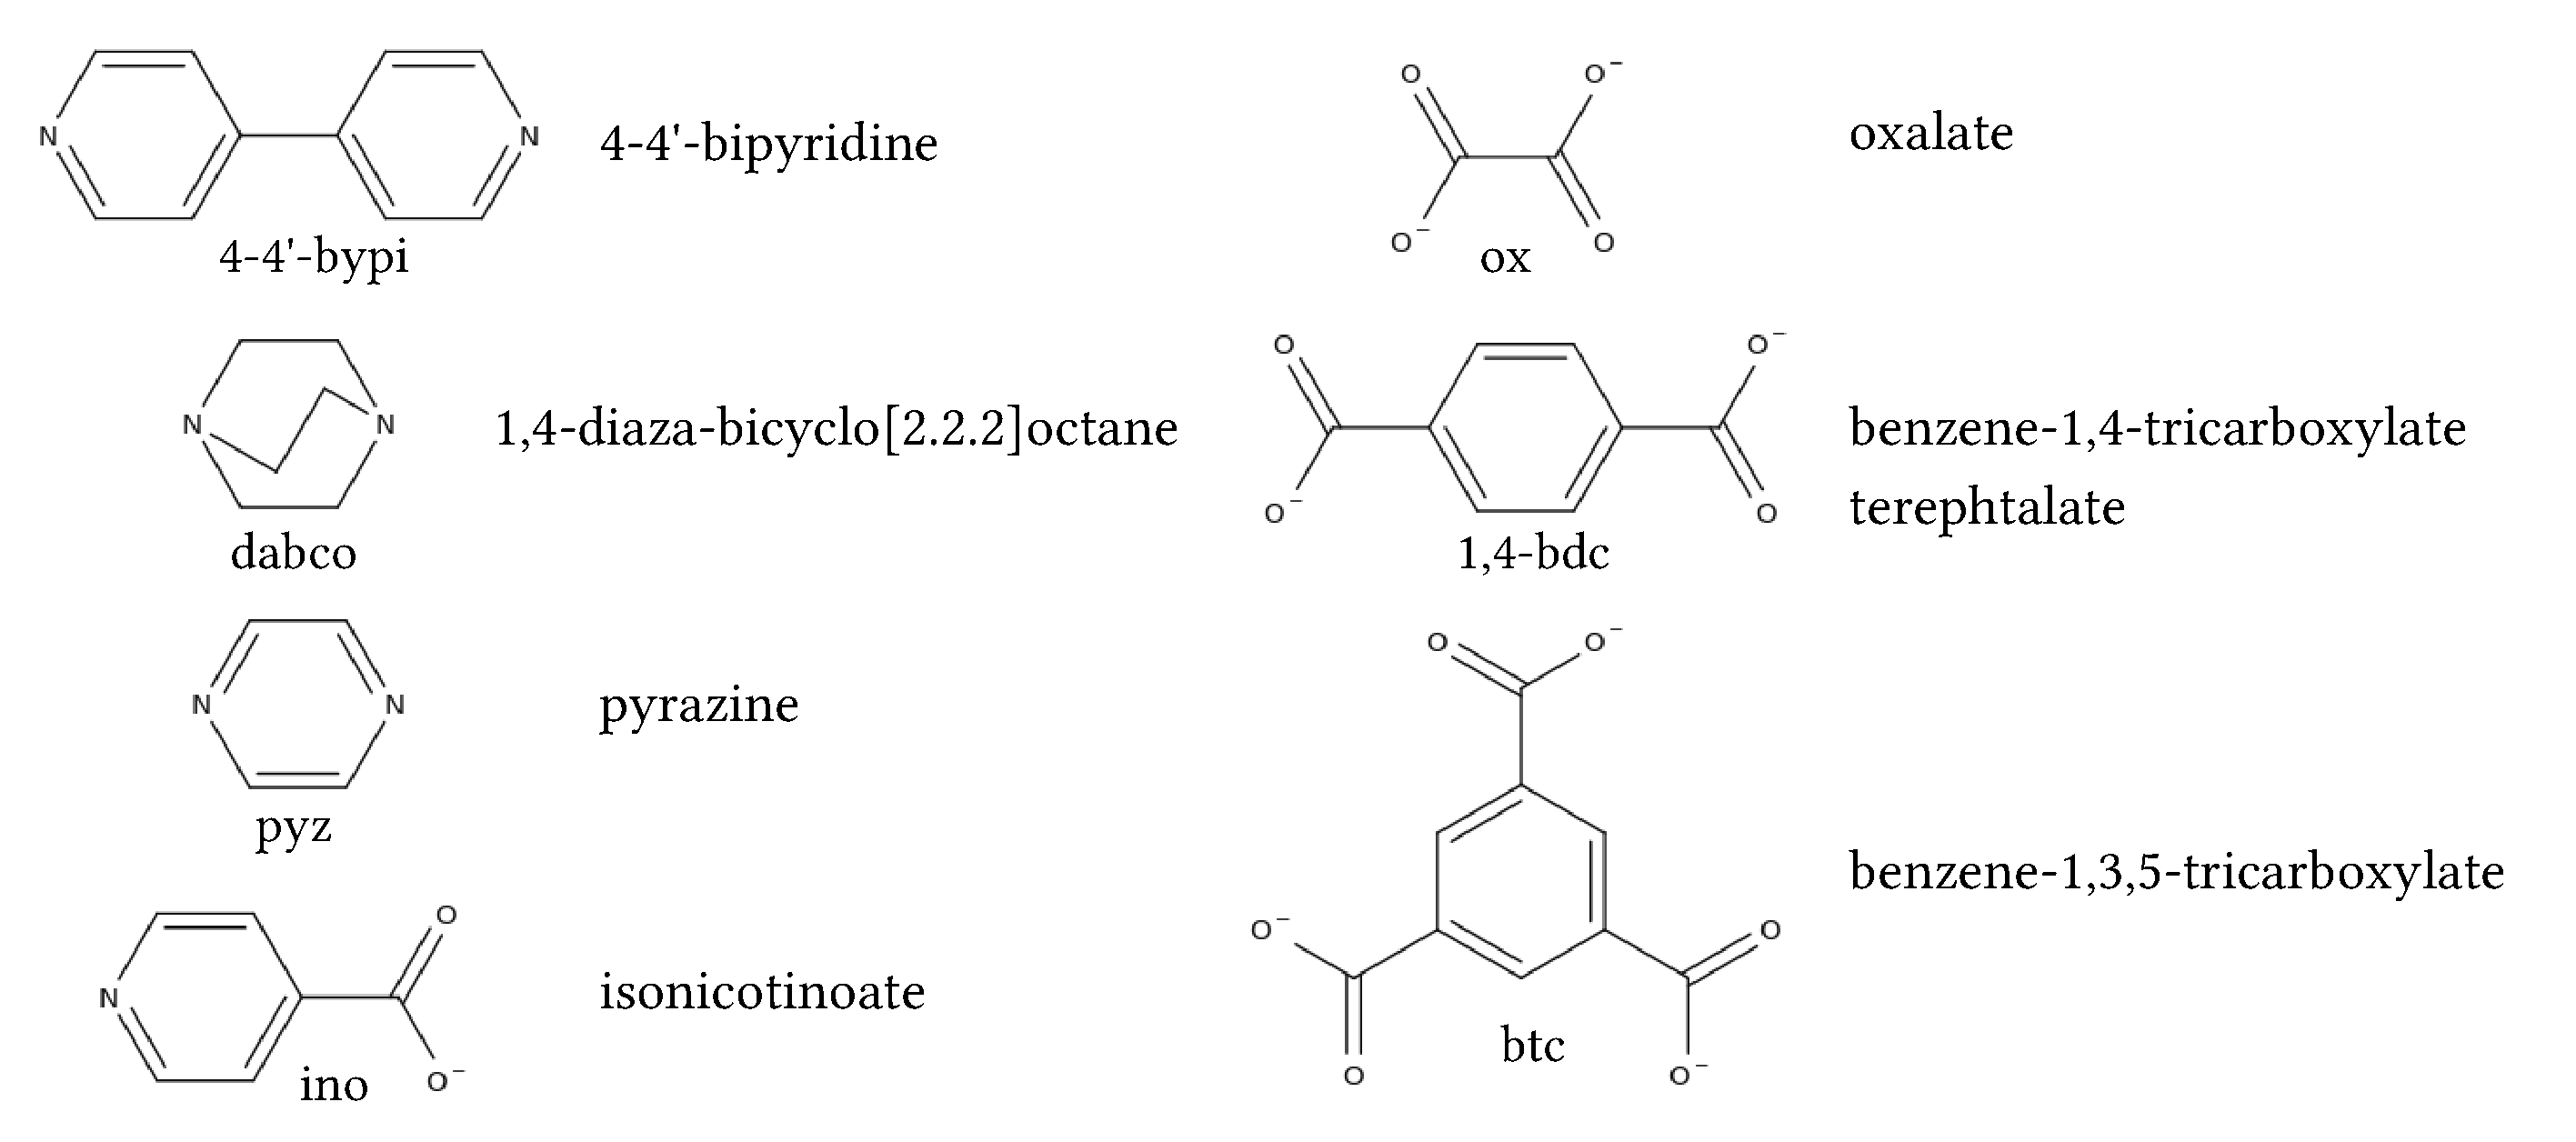
\includegraphics[width=\textwidth]{figures/images/mof-linkers}
    \caption{Frequently used linkers in MOF synthesis.}
    \label{fig:mof-linkers}
\end{figure}

\subsubsection{High structural diversity}

\begin{figure}[ht]
    \centering
    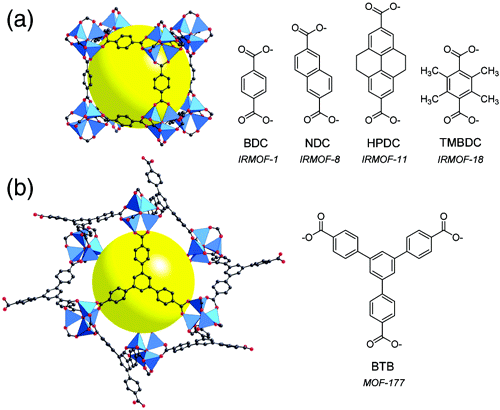
\includegraphics[width=0.6\textwidth]{figures/images/mof-different-linker}
    \caption{Examples of two MOFs built with a zinc oxide cluster with the same
    coordination geometry. (a) Structure of MOF-5, made with a linear linker.
    (b) Structure of MOF-177, made with a trigonal linker. Image from
    reference~\cite{Rowsell2004}.}
    \label{fig:mof-different-linkers}
\end{figure}

\begin{figure}[ht]
    \centering
    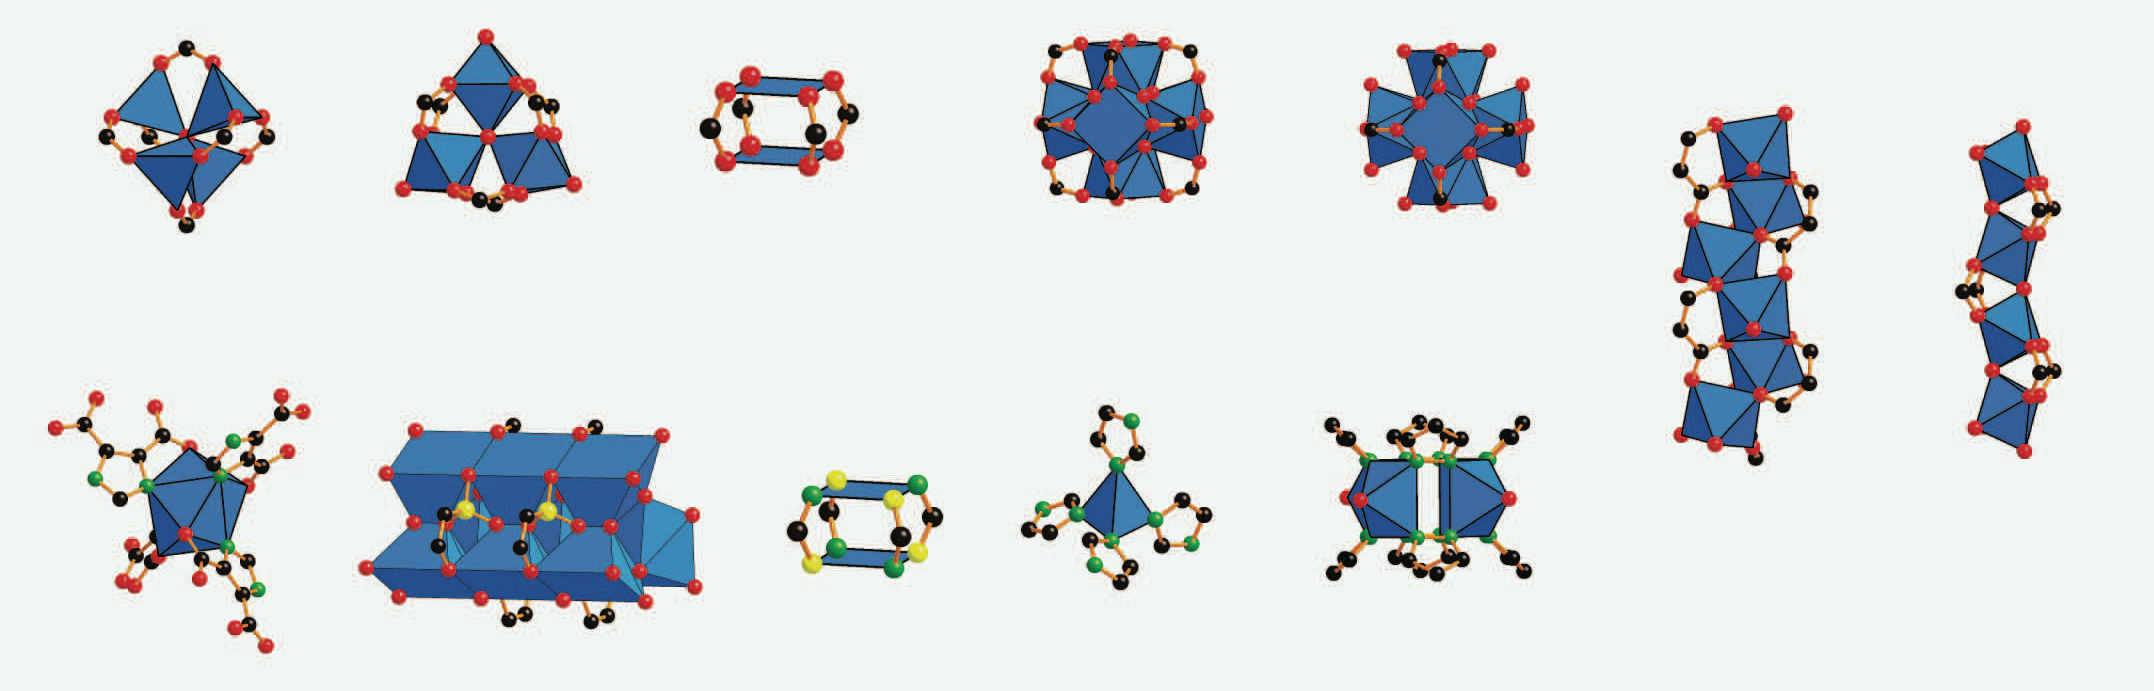
\includegraphics[width=\textwidth]{figures/images/mofs-sbu}
    \caption{Secondary building units examples. In blue we have metallic cation
    polyhedra, in red oxygen atoms, in black carbon atoms. Image from
    reference~\cite{Furukawa2013}.}
    \label{fig:mofs-sbu}
\end{figure}

\begin{figure}[htp]
    \centering
    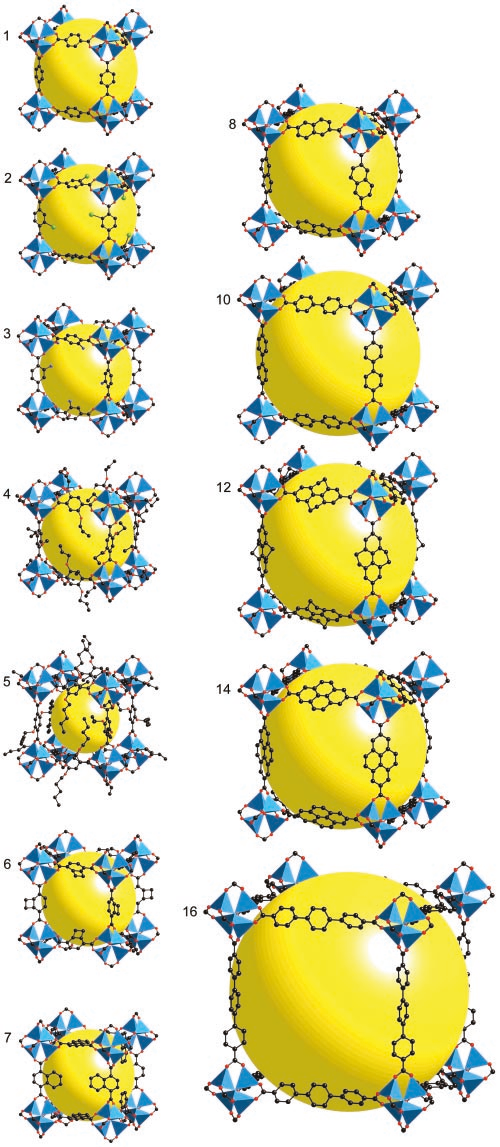
\includegraphics[width=0.4\textwidth]{figures/images/irmof-all-sizes}
    \caption{Structures of the IRMOFs-n (n = 1-8, 10, 12, 14, and 16). Zinc
    metallic polyhedra are in blue, carbon atoms in black, oxygen in red. The
    yellow sphere represent the porous volume of each structure. Image from
    reference~\cite{Eddaoudi2002}.}
    \label{fig:irmof-all-sizes}
\end{figure}

\subsubsection{Functionalization}

\subsection{Zeolitic Imidazolate Frameworks}

\begin{figure}[ht]
    \centering
    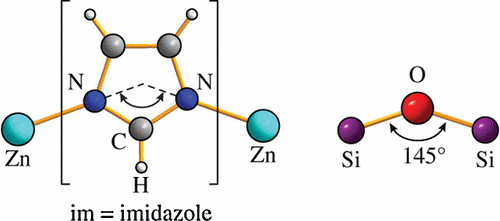
\includegraphics[width=0.4\textwidth]{figures/images/zeolite-to-zif}
    \caption{Illustration of the analogy between ZIFs and zeolite coordination.
    Image taken from reference~\cite{Bennett2010}}
    \label{fig:zeolite-to-zif}
\end{figure}

\begin{figure}[ht]
    \centering
    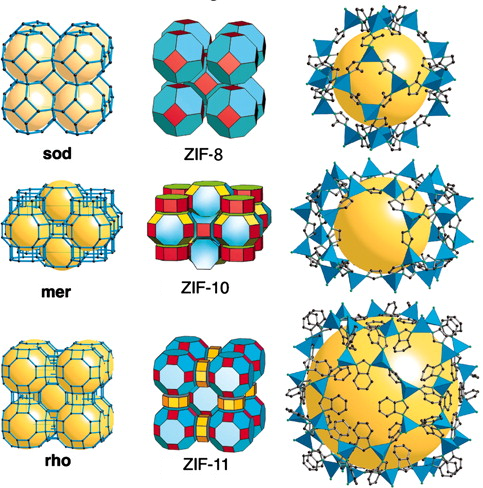
\includegraphics[width=0.6\textwidth]{figures/images/zif-examples}
    \caption{Three examples of ZIFs: ZIF-8, ZIF-10 and ZIF-11. From left to
    right are the crystalline structure of a zeolite with the same topology,
    the crystalline structure of the ZIF and the biggest sphere inside the
    cages. Image taken from reference~\cite{Park2006}}
    \label{fig:zif-examples}
\end{figure}

\subsection{Structural flexibility}

\begin{figure}[ht]
    \centering
    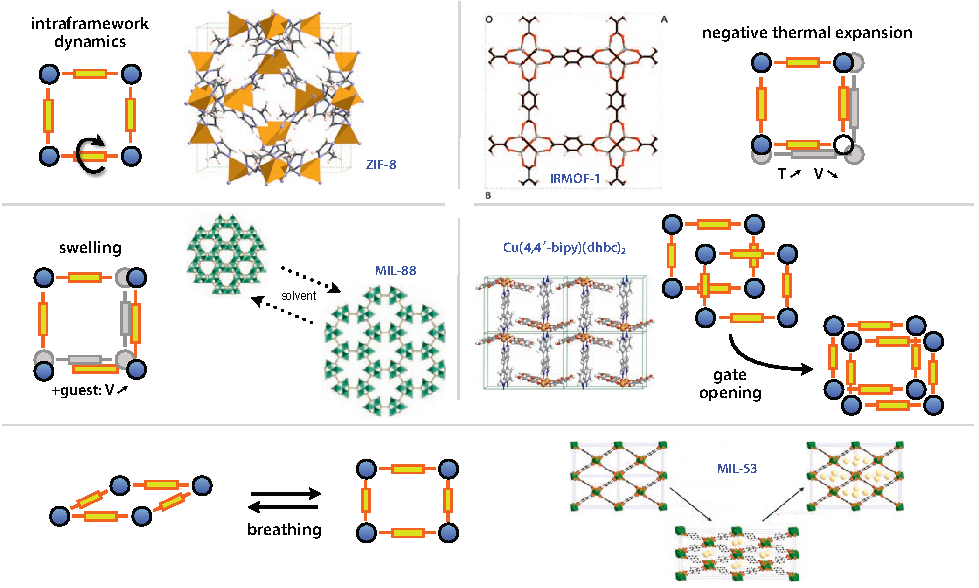
\includegraphics[width=\textwidth]{figures/images/mof-flexibility}
    \caption{Illustration of the main flexibility modes of MOFs: linkers
    rotation, thermal expansion, swelling, gate opening and breathing. Image
    taken from reference~\cite{Coudert2011}.}
    \label{fig:mof-flexibility}
\end{figure}

\subsection{Industrial applications}

% Among the porous materials used commercially, one can list
% inorganic materials (such as zeolites and silica gels), carbon-based compounds
% (e.g., activated carbon), and hybrid organic--inorganic materials, including the
% topical family of metal-organic frameworks or porous coordination polymers.

% \subsection{ZIF}
%
% ZIFs are built around tetravalent metal centers such as Fe, Co, Zn, Cd or Cu;
% linked together by imidazolate linkers.  They also present the same topology as
% zeolites, with metal(imidazolate)$_2$ building blocks taking the role of
% \ce{SiO2}. The first ZIFs (ZIF-1 to ZIF-12) were synthesized in
% 2006\cite{Park2006}, and found to be water and thermally resistant, which made
% them interesting MOF for commercial applications.

% Nanoporous crystalline materials such as zeolites, metal--organic frameworks
% (MOF), carbon nanotubes and inorganic open frameworks enjoy a wide range of
% applications, ranging from catalysis, fluid separation and purification, to gas
% capture and detection of dangerous molecules. The fundamental basis for most of
% these applications is the material's capability to adsorb large quantities of
% molecules inside its nanometer-sized pores, due to its large specific surface
% area.\cite{Rouquerol2013} In this context, hydrophobic nanoporous
% materials offer the advantage that the uptake of water from the gas phase ---
% e.g., humidity in the air --- is very small.\cite{Wu2010, Ghosh2013, Wang2016}
% Given that water is often strongly adsorbed and competes with other molecules
% for adsorption sites, hydrophobic molecular sieves can offer higher separation
% properties.\cite{Flanigen1978, Giaya2000}

% \ZIF8 is a nanoporous material part of the Zeolitic Imidazolate
% Frameworks (ZIF) family. These MOF are built from imidazolate anions as their
% organic linker (mim = 2-methylimidazolate in the case of \ZIF8) and a divalent
% metal cation (here, \ce{Zn^2+}). The frameworks of ZIFs are four-connected,
% meaning that the ZIFs adopt zeolitic topologies, with the metal center replacing
% the tetrahedral silicon atom and the linker replacing the oxygen atoms in the
% \ce{SiO2} building block. \ZIF8 has formula \ce{Zn(mim)2} and adopts the
% sodalite (\textbf{sod}) topology. In this topology, large quasi-spherical pores
% corresponding to the sodalite cages are connected by windows formed by 6 and 4
% zinc atoms (see figure~\ref{fig:SOD}). In \ZIF8, the 4 members windows are too
% small for any molecules to go through, and all of the connectivity of the pore
% space happens though the 6 members windows.

\newpage
\section{Adsorption and Intrusion}

\newpage
\section{Molecular simulations}

\subsection{Atoms and molecules}

\subsection{System size and periodic boundary conditions}

\OnlyInSubfile{\printbibliography}

\end{document}
